\documentclass[10pt]{article}

%% Various useful packages and commands from different sources

\usepackage[applemac]{inputenc}
\usepackage[english]{babel}
\usepackage[T1]{fontenc}
\usepackage{cite, url,color} % Citation numbers being automatically sorted and properly "compressed/ranged".
%\usepackage{pgfplots}
\usepackage{graphics,amsfonts}
\usepackage[pdftex]{graphicx}
\usepackage[cmex10]{amsmath}
\usepackage{bm}
% Also, note that the amsmath package sets \interdisplaylinepenalty to 10000
% thus preventing page breaks from occurring within multiline equations. Use:
 \interdisplaylinepenalty=2500
% after loading amsmath to restore such page breaks as IEEEtran.cls normally does.

% Compact lists
\usepackage{enumitem}
\usepackage{booktabs}
\usepackage{fancyvrb}

\usepackage{listings} % for Matlab code
\definecolor{commenti}{rgb}{0.13,0.55,0.13}
\definecolor{stringhe}{rgb}{0.63,0.125,0.94}
\lstloadlanguages{Matlab}
\lstset{% general command to set parameter(s)
framexleftmargin=0mm,
frame=single,
keywordstyle = \color{blue},% blue keywords
identifierstyle =, % nothing happens
commentstyle = \color{commenti}, % comments
stringstyle = \ttfamily \color{stringhe}, % typewriter type for strings
showstringspaces = false, % no special string spaces
emph = {for, if, then, else, end},
emphstyle = \color{blue},
firstnumber = 1,
numbers =right, %  show number_line
numberstyle = \tiny, % style of number_line
stepnumber = 5, % one number_line after stepnumber
numbersep = 5pt,
language = {Matlab},
extendedchars = true,
breaklines = true,
breakautoindent = true,
breakindent = 30pt,
basicstyle=\footnotesize\ttfamily
}

\usepackage{array}
% http://www.ctan.org/tex-archive/macros/latex/required/tools/
\usepackage{mdwmath}
\usepackage{mdwtab}
%mdwtab.sty	-- A complete ground-up rewrite of LaTeX's `tabular' and  `array' environments.  Has lots of advantages over
%		   the standard version, and over the version in `array.sty'.
% *** SUBFIGURE PACKAGES ***
\usepackage[tight,footnotesize]{subfigure}
\usepackage[top=2.2cm, bottom=2.2cm, right=1.7cm,left=1.7cm]{geometry}
\usepackage{indentfirst}


%\setlength\parindent{0pt}
\linespread{1}

\usepackage{mathtools}
\DeclarePairedDelimiter{\ceil}{\lceil}{\rceil}
\DeclarePairedDelimiter{\floor}{\lfloor}{\rfloor}
\DeclareMathOperator*{\argmax}{arg\,max}
\newcommand{\M} {\mathtt{M}}
\newcommand{\dB} {\mathrm{dB}}
\newcommand{\tr} {\mathrm{tr}}
\newcommand{\ofdM} {\mathcal{M}}
\newcommand{\DFTmat} {\mathcal{\boldsymbol{F}}}
\newcommand{\lmod}[1] {_{\,\mathrm{mod}\,#1}}



\graphicspath{ {figures/} }

% equations are numbered section by section
%\numberwithin{equation}{section}


\begin{document}
\title{Digital Transmission - Homework 4}
\author{Andrea Dittadi, Davide Magrin, Michele Polese}

\maketitle

%%%%%%%%%%%%%%%%%%%%%%%%%%%%%%%%%%%%%%%%%
%%%%%%%%%%%%%% PROBLEM 1 %%%%%%%%%%%%%%%%
%%%%%%%%%%%%%%%%%%%%%%%%%%%%%%%%%%%%%%%%%

\section*{Problem 1}

% Description of system setup

\begin{figure}[h!]
	\centering
	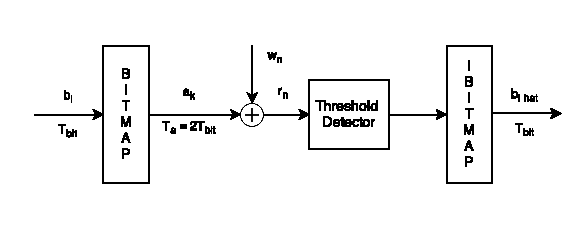
\includegraphics[width = 0.8\textwidth]{SC_uncoded}
	\caption{Block diagram for the simulation of a Single Carrier uncoded QPSK}
	\label{fig:problem1_scuncoded}
\end{figure}

\begin{figure}[h!]
	\centering
	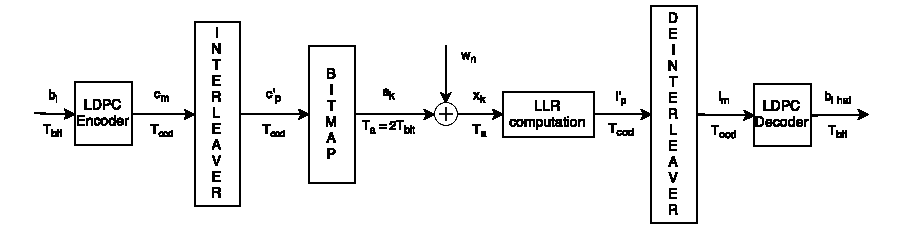
\includegraphics[width = \textwidth]{SC_coded}
	\caption{Block diagram for the simulation of a Single Carrier coded QPSK}
	\label{fig:problem1_sccoded}
\end{figure}

The uncoded Single Carrier QPSK configuration was implemented as described in Figure~\ref{fig:problem1_scuncoded}. First of all, a random data stream is created using the \texttt{randi} function. For the Pbit simulations, $L_{bits} = 2^{24}$ bits were used for every SNR. While this number of bits is unnecessarily large to estimate the Bit Error Rate for the lower SNRs, it was decided not to optimize it because the simulations were sufficiently fast. This is due to the lightweight operations the script has to perform: after the initial bitmapping of the bits to obtain the QPSK symbols, the channel only adds noise and there is no need to perform any convolution with an impulse response since the channel is ideal. Finally, the receiver only computes a thresholding and an inverse bit mapping. The results of the simulation can be seen in Figure~\ref{fig:problem1_pbit}, and coincide with those obtained in the previous homework. % TODO insert this reference to the old homework???

When using coding, the script has to perform more complex computations that are illustrated in Figure~\ref{fig:problem1_sccoded}. The random bit sequence needs to have a length compatible with both the encoder and the interleaver. In fact, the provided LDPC encoder requires information words to have length $L_{iw} = 32400$ bits, and encodes them into codewords of length $L_{cw} = 64800$ bits. This doesn't represent a limitation, as shorter information words may be padded to reach the desired length, encoded and de-padded at the receiver, once decoded. In order to simplify things, however, it was decided to only send information words that have length that is a multiple of the information word length required by the encoder. Additionally, the interleaver matrix was given dimensions of 30 x 36 in order to facilitate the process of interleaving the codeword bits. Since $30 \cdot 36 = 1080$ is a divisor of the length of the codewords outputted by the encoder, when codewords of length $L_{cw} = k \cdot 64800, k \in \mathbb{N^{+}}$ need to be interleaved, the interleaver uses a number of matrices equal to $\frac{L_{cw}}{30\cdot36} = 60 \cdot k$, thus ensuring that all matrices will be filled completely and that no additional padding is required. Using this setup, if the desired length is $L_d$, the nearest compatible length of the message to be sent can be computed using the expression $L_{msg} = \lceil \frac{L_{d}}{32400} \rceil \cdot 32400$.

% Expressions of LLRs l'_2k and l'_(2k+1)

% BER plot for coded vs uncoded QPSK
\begin{figure}
	\centering
	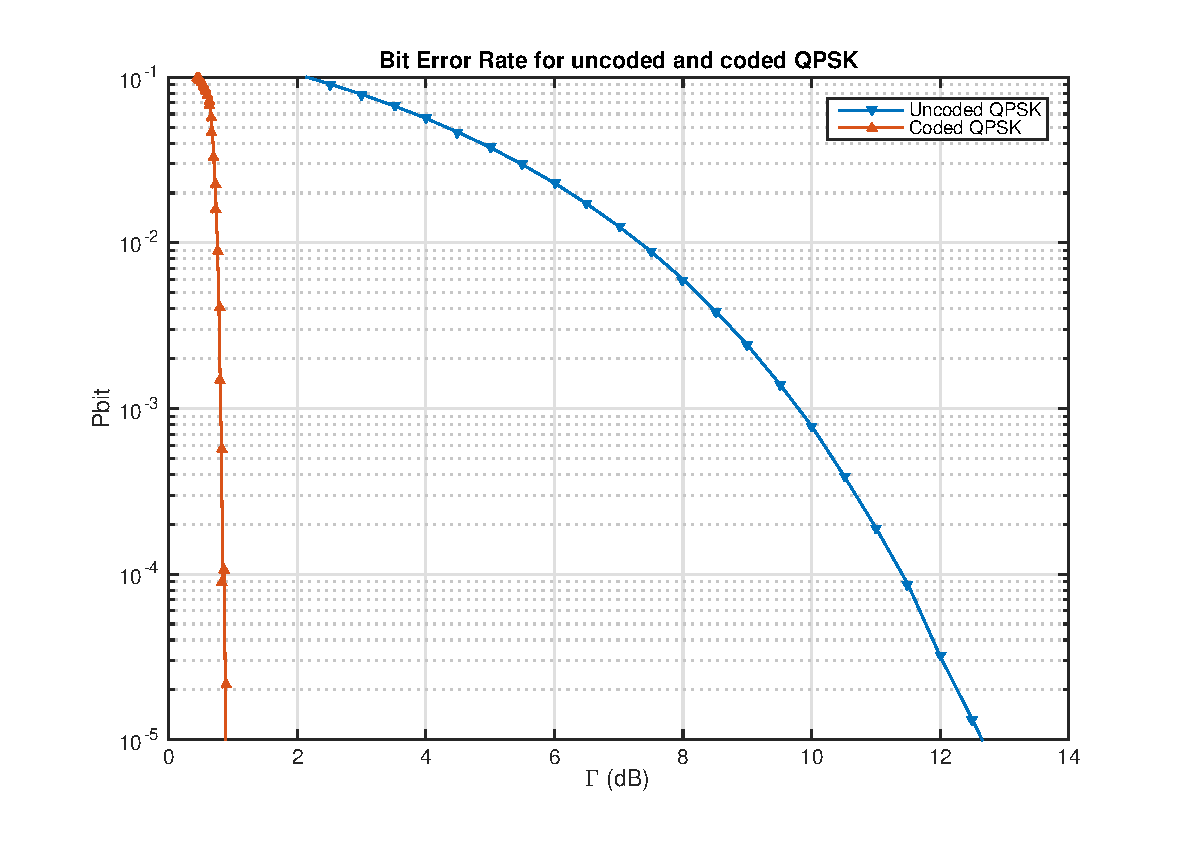
\includegraphics[width = 0.8\textwidth]{problem1}
	\caption{BER simulation results for coded vs. uncoded QPSK}
	\label{fig:problem1_pbit}
\end{figure}



%%%%%%%%%%%%%%%%%%%%%%%%%%%%%%%%%%%%%%%%%
%%%%%%%%%%%%%% PROBLEM 2 %%%%%%%%%%%%%%%%
%%%%%%%%%%%%%%%%%%%%%%%%%%%%%%%%%%%%%%%%%

\section*{Problem 2}

%%%%%%%%%%%%%%%%%%%%%%%%%%%%%%%%%%%%%%%%%
%%%%%%%%%%%%%% PROBLEM 2 %%%%%%%%%%%%%%%%
%%%%%%%%%%%%%%%%%%%%%%%%%%%%%%%%%%%%%%%%%
\section*{Problem 3}

\subsection*{Transmitter structure}

% cyclic prefix
% idft
% p/s
% This consideration on SNR
As usual the SNR is defined as $\Gamma = \frac{\sigma_s^2 E_h}{\sigma_w^2}$. With an OFDM system, however, the meaning of $\sigma_s^2$ changes. In particular if the transmitter is implemented with an IDFT, which is
\begin{equation}
	A_k[\ell] = \frac{1}{\ofdM} \sum_{i = 0}^{\ofdM - 1} W_{\ofdM}^{-i\ell} a_k[i], \quad \ell = 0, 1, \dots, \ofdM-1
\end{equation}
followed by the polyphase compoment of a prototype filter, which in our case is a $\delta_n$ filter, with a gain $\ofdM$ as specified in \cite{bc}, then we have 
% see formula 9.35, 9.38, 9.39
\begin{equation}
	\sigma_s^2 = \sigma_a^2
\end{equation}
since data is IID. 

However, since the gain factor would simply change the scaling of the data and should be removed at the receiver, we don't consider it in the actual implementation. MATLAB \texttt{ifft} performs the IDFT with the correct scaling factor of $1/\ofdM$. Therefore, if the energy of the data symbols that are pushed into the channel is considered, then
\begin{equation}
	\Gamma = \frac{\sigma_a^2 E_h}{\ofdM \sigma_w^2}
\end{equation}
must be the SNR considered when computing the noise level introduced by the channel in our implementation.


\subsection*{Receiver structure}
% TODO add figure as in line below
The receiver of OFDM has the structure of Figure. The timing phase is $t_0 = 5 T$, which corresponds to the beginning at the receiver of the cyclic prefix. For each block of $\ofdM + N_{px}$ symbols the first $N_{px}$ are discarded and the DFT is then computed only on the $\ofdM$ samples which don't belong to the cyclic prefix of each block. Let the vector of symbols before the DFT be $\mathbf{r}_k$, with $k$ the block index, and $\mathbf{g}_{c,\ofdM}$ be the channel impulse response, of length $N \le N_{px} - 1$, padded with zeros in order to have a vector of length $M$. Then it is possible to define the circulant matrix of the IDFT of the transmitted symbols $a_k[i], i = 0, \dots, \ofdM$ as
\begin{equation}
	\boldsymbol{\Xi} = 
	\begin{bmatrix}
		A_k[0] & A_k[\ofdM - 1] & \dots & A_k[1] \\
		A_k[1] & A_k[0] & \dots & A_k[2] \\
		\vdots & \vdots & \ddots & \vdots \\
		A_k[\ofdM - 1] & A_k[\ofdM - 2] & \dots & A_k[0] \\
	\end{bmatrix}
\end{equation}
and express $\mathbf{r}_k$ as
\begin{equation}
	\mathbf{r}_k = \boldsymbol{\Xi} \mathbf{g}_{c,\ofdM} + \mathbf{w}_k
\end{equation}
with $w_k$ a vector of AWGN samples. Then the receiver performs the DFT using an $\ofdM \times \ofdM$ DFT matrix $\DFTmat$ in order to get $ \mathbf{x}_k = \DFTmat \mathbf{r}_k$. In particular, let's consider the following 
\begin{eqnarray}
	 \mathbf{x}_k & = & \DFTmat \mathbf{r}_k = \DFTmat \boldsymbol{\Xi} \DFTmat^{-1} \DFTmat \mathbf{g}_{c,\ofdM} + \DFTmat \mathbf{w}_k\\
	  & = & \mathrm{diag}\{\mathbf{a}_k\} \mathbf{G}_c + \mathbf{W}_k
\end{eqnarray}
because $\boldsymbol{\Xi}$ is a circulant matrix. $W_k$ is a still a vector of independent Gaussian random variables, each of them with variance $\sigma_W^2 = \ofdM \sigma_w^2$. 

This procedure removes the effects of ICI and ISI introduced by the non-ideal channel, and it is followed by a scaling of the received symbols on each channel in order to get the same constellation of the transmitter. In particular for each subchannel $i$ 
\begin{equation}
	y[i] = \frac{x[i]}{G_c[i]} = a_k[i] + \frac{W_k[i]}{G_c[i]}
\end{equation}
Finally the receiver performs a decision. If the transmitted bits are uncoded, it uses a threshold detector on each subchannel and an inverse bitmap. Note that the performances of an uncoded OFDM system are negatively affected by the presence of subchannels in which the frequency response $G_c$ of the channel exhibits a great attenuation, because in that subchannels the received symbols are zeros or below noise level. 
% TODO fix this sentence

If the coded option is used, instead, the data which would be lost because of frequency response attenuation in that subchannel can be recovered with coding. In particular given the observed symbol $y_k[i]$ the log-likelihood ratios (LLR) of each subchannel are defined as
\begin{eqnarray}
	\mathrm{LLR}_I = \frac{2\mathrm{Re}(y_k[i])}{0.5\sigma_W^2/|G_c[i]|^2} = \frac{2\mathrm{Re}(y_k[i]) |G_c[i]|^2 }{0.5 M \sigma_w^2} \\
	\mathrm{LLR}_Q = \frac{2\mathrm{Im}(y_k[i])}{0.5 \sigma_W^2/|G_c[i]|^2} = \frac{2\mathrm{Im}(y_k[i]) |G_c[i]|^2 }{0.5 M \sigma_w^2} \\
\end{eqnarray}
since $0.5 \sigma_W^2/|G_c[i]|^2$ is variance per component of the noise of $y_k[i]$ for each subchannel.

\subsection*{Channel estimation for OFDM}
In order to perform the operations described in the previous section, the receiver has to know the frequency response of the channel and the noise power of each subchannel. In this homework the simulation of the BER has been carried out both with an a-priori perfectly known channel and with an estimated channel. 

%% TODO give reasons behind this kind of spacing
The estimation of the channel had to be performed with 32 pilot symbols, all in block $0$. For a given SNR $\Gamma$ computed with the data power $\sigma_a^2 = 2$, then the pilot symbols have $s\sigma_{ts} = 4$ as required. The pilot symbols were inserted in the subchannels $i \in \mathcal{T}_{ind} = \{ 0, 15, 31, \dots, 497 \}$, i.e. with a spacing of $\ofdM/32$ subchannels between each other. The other $\ofdM - 32$ symbols can be data or anything else, they are not used for the estimation. At the receiver at first the 32 $x_0[i], i \in \mathcal{T}_{ind}$ are divided by the corresponding pilot symbol in order to get $\tilde{G}[i] = G_c[i] + W_0[i]$. Then the procedure exploits the fact that the channel impulse response can have at most $N \le N_{px} + 1 = 8$ taps, so the uncorrelated samples of the $G_c[i]$ are at most 8. In particular if $\mathbf{G}_c$ is seen as the DFT of the channel impulse response then
\begin{equation}
	\mathbf{G}_c = \DFTmat_{\ofdM \times \ofdM} \mathbf{g}_{c,\ofdM} = \DFTmat_{\ofdM \times N_{px} + 1} \mathbf{g}_c
\end{equation}
By choosing the 32 subchannels in the proper way (i.e. for $ i\ \in \mathcal{T}_{ind}) $) it is possible to define a matrix $\boldsymbol{\tilde{\mathcal{F}}}$ of size $32 \times N_{px} + 1$ with the first $N_{px} + 1$ columns of $\DFTmat_{\ofdM \times \ofdM}$ (at most the ones which are not multiplied by zero), at rows $ i\ \in \mathcal{T}_{ind} $. Let $\tilde{W}_0$ be the vector of noise samples which correspond to the subchannels with pilot symbols. Then it is possible to write $\mathbf{\tilde{G}}_i = \tilde{G}[i], i\ \in \mathcal{T}_{ind}$ as
% TODO fix notation, put a different notation for real "received" G and their theoretical form
\begin{equation}
	\mathbf{\tilde{G}} = \boldsymbol{\tilde{\mathcal{F}}}\mathbf{g}_{c} + \tilde{W}_0
\end{equation}
The vector $\mathbf{g}_{c}$ can be finally found by applying the LS method on the system
\begin{equation}
% TODO write this in a better way, see the prev.TODO
	\boldsymbol{\tilde{\mathcal{F}}}\mathbf{g}_{c} = \mathbf{\tilde{G}}
\end{equation}
which is
\begin{eqnarray}
	\boldsymbol{\Phi} = \boldsymbol{\tilde{\mathcal{F}}}^H \boldsymbol{\tilde{\mathcal{F}}} \\
	\boldsymbol{\theta} = \boldsymbol{\tilde{\mathcal{F}}}^H \mathbf{\tilde{G}} \\ %% TODO this last factor should be the "observed" vector
	\hat{\mathbf{g}}_{c} = \boldsymbol{\Phi}^{-1} \boldsymbol{\theta} 
\end{eqnarray}


\begin{thebibliography}{10}

\bibitem{bc}
Benvenuto, Cherubini, Algorithms for Communications Systems and their Applications, Wiley, 2004

\end{thebibliography}

\end{document}
